\paragraph{Performance metrics.}
We use \emph{balanced accuracy} 
as our primary performance metric.
The class imbalance in TMED2 means standard accuracy is less suitable~\citep{huang2021new}.  
Given a dataset of $N$ true labels $y_{1:N}$ and $N$ predicted labels $\hat{y}_{1:N}$, with each AS diagnosis label in $\{0, 1, 2\}$, we compute balanced accuracy as $\sum_{c=0}^{2} \frac{\text{TP}_{c}(y_{1:N}, \hat{y}_{1:N})}{N_{c}(y_{1:N})}$, where $\text{TP}_c(\cdot)$ counts \emph{true positives} for class $c$ and $N_c(\cdot)$ counts all examples with class label $c$.
Later evaluations of screening potential assess discrimination between two classes via \emph{area under the ROC curve}.

%\begin{align}
%\text{balanced-accuracy}(y_{1:N}, \hat{y}_{1:N}) &= 
%\frac{1}{C} \sum_{c=1}^{C} \frac{\text{TP}_{c}(y_{1:N}, \hat{y}_{1:N})}{N_{c}(y_{1:N})}.
%\label{eq:balanced_accuracy}
%\end{align}
%Let $\text{TP}_c(\cdot)$ count \emph{true positives} for class $c$ (that is, the number of correctly classified examples whose true label is $c$), and $N_c(\cdot)$ gives the total number of examples with true label $c$. 



\paragraph{Comparisons.}
We compared our methods with a set of strong baseline including general-purpose multiple-instance learning algorithms ~\citep{zaheer2017deep, ilse2018attention, lee2019set, li2021dual} and prior methods for Aortic Stenosis diagnosis using deep neural networks ~\citep{wessler2023automated, holste2022automated, holste2022self}. %Results are shown in Table \ref{tab:TMED2_BACC}. 
We also tried DeepSet, but omit those results as we were not able to perform better than random chance on this challenging diagnostic task despite substantial hyperparameter tuning (details in App.~\ref{App:DeepSet}).

%We did not show DeepSet in Tabel \ref{tab:TMED2_BACC}, because  despite substantial effort on hyperparameter tunning, we wouldn't able train DeepSet to obtain meaningful result. More details can be found in App ~ . 
%This again demonstrates how challenging the problem of diagnosing AS from ultrasound image is. 

% \todo{Another general-purpose \footnote{Although DSMIL is purposed mainly for WSI classification, the author claimed that the method also work well on general MIL problems} state-of-the-art deep MIL method is DSMIL~\citep{li2021dual}. We didnt' compare with DSMIL since we found that two of the three key components: multi-scale fusion and identifying key instances from max-pooling then calculate attention weight of each instance based on the distance to the key instance, are inappropriate for our problem if apply directly without substantial modification.}    

\begin{table}[!t]
    \begin{tabular}{l|rrr| r | r r}
	    & \multicolumn{4}{c}{Test Set Bal. Accuracy} & & \\
     Method & split 1 & split 2 & split 3 & average & \# params & view clf.?\\
    \hline
    Filter then Avg. [b] & 62.06 & 65.12 & 70.35 & 65.90 & 11.18 M & Yes
    \\
    W. Avg. by View Rel. [c]$*$
    & 74.46 & 72.61 & 76.24 & 74.43 &  5.93 M & Yes
    \\
    %JASE  & 11.87 M & 74.46 & 72.61 & 76.24 & 74.43 & Yes\\
    %Yale  & 11.18 M & 62.06 & 65.12 & 70.35 & 65.90 & Yes\\
    SAMIL (ours)            & 75.41 & 73.78 & 79.42 & \textbf{76.20}& 2.31 M & No
    \\
    \hline
    ABMIL [d]                 & 58.51 & 60.39 & 61.61 & 60.17 & 2.25 M & No\\
    ABMIL + Gate Attn. [d]  & 57.83 & 62.60 & 59.79 & 60.07 & 2.31 M & No \\
    Set Transformer [e]  & 60.95 & 62.61 & 62.64 & 62.06&  1.98 M & No \\
    DSMIL [f]  & 60.10 & 67.59 & 73.11 & 66.93&  2.02 M & No \\
    % VR ABMIL (ours)  & 2.31 M & 72.72 & 71.60 & 73.46 & 72.59& No \\
    \end{tabular}
    \\
    % {\small [b] \citet{holste2022automated}, [c] \citet{wessler2023automated} 
    %  [d] \citet{ilse2018attention} [e] \citet{lee2019set} [f] \citet{li2021dual} 
    % }%end citation list
     {\footnotesize [b] \citet{holste2022automated}, [c] \citet{wessler2023automated} 
     [d] \citet{ilse2018attention} [e] \citet{lee2019set} [f] \citet{li2021dual} 
    }%end citation list
    \caption{AS diagnosis results on TMED2. Showing balanced accuracy (percentage, higher is better) on the test set across three train/test splits. Methods b, c, d are diagrammed in corresponding panel in Fig.~\ref{fig:diagrams}.
    Methods above the line are approaches specialized to the AS task, others are generic MIL methods. Column ``\# params'' shows number of trainable parameters. Column ``view clf.?'' shows whether an additional view classifier is needed at deployment. $*$: value from the cited paper.
    }%endcaption
    \label{tab:TMED2_BACC}
\end{table}

\subsection{Quantitative evaluation on TMED-2}
Table \ref{tab:TMED2_BACC} compares all methods on test-set balanced accuracy for AS diagnosis (3 levels, no/early/significant) across the 3 splits of TMED2.
%In the results shown in Table \ref{tab:TMED2_BACC},
Our proposed method, SAMIL, scores 76\%, signficantly better than other state-of-the-art attention-based MIL architectures we tested (which span 60-67\%). 
SAMIL improves over its predecessor ABMIL by a remarkable \textbf{16\%} gain, 
which is consistent across splits.
%When compared to ABMIL, upon which SAMIL is built, our method achieves a remarkable performance gain of over \textbf{16\%}, with consistent gains across all three splits.
SAMIL also outperforms more recent MIL architectures like Set Transformer, which employs self-attention for both feature extraction and pooling, and the recent state-of-the-art DSMIL, which leverages a two-stream architecture. 
%Despite SAMIL's conceptual simplicity, it performs notably better: approximately \textbf{14\%} better than Set Transformer and \textbf{9\%} better than DSMIL.

Table \ref{tab:TMED2_BACC} also compares recent dedicated AS diagnostic models, revealing that our SAMIL method achieves better performance at substantially \emph{smaller model size}. Moreover, once trained, our model can process the entire TTE study (dozens of images of different views) without the need to deploy an additional view classifier to filter \citep{holste2022automated,holste2022self} or downweight \citep{wessler2023automated} images. This highlights the efficiency and effectiveness of SAMIL in comparison to other approaches.

To understand the source of SAMIL's gains, we provide confusion matrices in Fig.~\ref{fig:confusion_matrix}.
%comparing it to W. Avg. by View Rel ~\citep{wessler2023automated} DSMIL ~\citep{li2021dual} and ABMIL~\citep{ilse2018attention}. 
SAMIL outperforms W. Avg. by View Rel. in early AS recall, while maintaining similar or slightly lower no AS and significant AS recall. Compared to DSMIL, SAMIL improves no AS and early AS recall, with similar significant AS recall. Compared to ABMIL, SAMIL performs better in all three categories.

% Compared to W. Avg. by View Rel, SAMIL achieves better recall for early AS while being on par or slightly worse on recall for no AS and Significant AS. Compared to DSMIL, SAMIL achieve better recalls on no AS and early AS, while being on par on significant AS. Compared to ABMIL, SAMIL achieves better recall for all the three categories.  

%\subsection{Using Automatic Study-Level Diagnosis as a Preliminary Screening Tool for AS}

Fig~\ref{fig:TMED2_roc} shows ROC curves indicating discriminative performance of three clinical use cases for binary screening (no vs some AS, early vs significant, and significant AS vs not). SAMIL outperforms ABMIL and DSMIL across all tasks. 
In comparison to W. Avg. by View Rel, SAMIL reaches similar performance in screening No AS vs. Some AS, while doing better in the other two tasks.

% Discriminatory performance for various clinical use cases are shown in Fig~\ref{fig:TMED2_roc}. SAMIL performs significantly better than ABMIL and DSMIL on all three tasks. Compared to W. Avg. by View Rel, despite being smaller in model size, SAMIL achieves comparable performance on No AS vs Some AS, while clearly better at Early vs Significant and No Significant vs Significant tasks.


\subsection{Evaluation of screening potential on 2022-Validation set.}
We further validate methods on the separate 2022-Validation dataset described earlier, which contains 225/48/50 examples of no/early/significant AS. 
Results in Tab.~\ref{tab:AUC_analysis_323}
compare SAMIL to the best-performing baselines from previous section. 
SAMIL achieved competitive performance on two critical screening tasks: It seems best on Significant-vs-Not and equivalent to the best on No-vs-Some. On the more challenging Early-vs-Significant, where both classes have 50 or fewer examples in this set, all methods have wide uncertainty intervals from bootstrap resamples of this test set, and SAMIL remains only a bit behind DSMIL.

%Note that the early-vs-significant task has especially wide uncertainty intervals due to the small number of available cases (9) of early AS.

% \begin{table}[h]
% \centering
% \begin{tabular}{c|c|c|c}
%        & \multicolumn{3}{c}{AUROC for AS screening}
%        \\
% Method & No vs Some & Early vs Significant & Significant vs. Not \\
% \hline
% W. Avg. by View Rel.  & 0.948 (0.898, 0.980)  & 0.582 (0.312, 0.829) & 0.909 (0.859, 0.949)
%  \\
% DSMIL.  & 0.899 (0.839, 0.945)  & 0.881 (0.730, 0.991) & 0.941 (0.893, 0.978)\\
% SAMIL (ours) & 0.935 (0.867, 0.978)  & 0.805 (0.645, 0.931) & 0.958 (0.923, 0.983) \\

% \end{tabular}
% \caption{AUROC for AS screening on temporarily distinct cohort. Values in parenthesis show 2.5th and 97.5th percentiles of AUROC values computed from 5000 bootstrap resamples of 263 studies.}
% \label{tab:AUC_analysis_263}
% \end{table}

\begin{table}[h]
\centering
\begin{tabular}{c|c|c|c}
       & \multicolumn{3}{c}{AUROC for AS screening}
       \\
Method & No vs Some 
    & Significant vs. Not
    & Early vs Significant 
    \\
\hline
W. Avg. by View Rel.  & 0.934 (0.904, 0.959)  
    & 0.881 (0.837, 0.921)
    & 0.653 (0.539, 0.760) 
 \\
DSMIL.  & 0.897 (0.862, 0.929)  
    & 0.902 (0.857, 0.941)
    & 0.765 (0.664, 0.857) 
    \\
SAMIL (ours) & 0.923 (0.885, 0.955)  
    & 0.921 (0.886, 0.951) 
    & 0.717 (0.610, 0.813) 
    \\
\end{tabular}
\caption{AUROC for AS screening on temporarily distinct cohort. Values in parenthesis show 2.5th and 97.5th percentiles of AUROC values computed from 5000 bootstrap resamples of 323 studies.}
\label{tab:AUC_analysis_323}
\end{table}


\subsection{Assessment of attention quality}

Our supervised attention module is intended to ensure that the model's decision-making process is consistent with human expert intuition, by only using relevant views to make diagnostic judgments.
Here, we evaluate how well the attention mechanisms of various models align with this goal. 
Fig \ref{fig:Attention_View_Alignment} compares the predicted view relevance of SAMIL's and ABMIL's attended images, aggregating across all studies in the test set. For instance, the first panel reveals that after ranking by attention, the 9th ranked image by ABMIL on average has less than 0.5 view relevance. This means that for many studies, some images in the top 9 (as ranked by attention) are likely from irrelevant views. In contrast, SAMIL's 9th ranked image has an average view relevance above 0.9.
Overall, the figure demonstrates that SAMIL bases decisions on clinically relevant views, while ABMIL fails this clinical sanity check. 
We hope these evaluations reveal how our SAMIL's improved attention module contributes to helping audit a model's overall interpretability, which is key to gaining trust from clinicians and successfully adopting an ML system in medical applications ~\citep{holzinger2017we, lundberg2017unified, tonekaboni2019clinicians}. 

%In addition to achieving superior performance, our proposed method enhances the interpretability and trustworthiness of the model compared to standard off-the-shelf MIL models. 

% Fig ~\ref{fig:Attention_View_Alignment} compares the predicted view relevance of each attended images of SAMIL with those of ABMIL. This visual shows an aggregated perspective across all studies in the test set. For example, in split 1, the top 9th attended images across all studies, on average only has a predicted view relevance of less than 0.5. This indicates that for many studies in this test split, the 9th attended images by ABMIL is likely from \textbf{irrelevant views}. On the other hand, for the same figure, the top 9th attended images by SAMIL has an average predicted view relevance of above 0.9, which substaintially higher than that of the ABMIL (0.5), indicating that these attended images by SAMIL are very likely to from relevant views. The figure as a whole, demonstrates that SAMIL makes decisions based on clinically relevant views, while ABMIL fails the clinical sanity check.

We provide two additional sanity checks for our supervised attention module. 
First, Fig ~\ref{fig:top_attended_images} illustrates the top 10 images ranked by attention from one study (the first in the test set to avoid cherry-picking).
Among the top 10 images attended by ABMIL, 5 are actually irrelevant views. In contrast, the top 10 images attended by SAMIL are all from relevant views.
Second, we assess the view classifier's performance on the view classification task in App~\ref{app:ViewClassifier}, supporting that its predicted view relevance serves as a reliable indicator for assessing whether an image comes from a relevant view or not.

\setlength{\tabcolsep}{0.1cm}
\begin{figure}
\begin{tabular}{c c c }
     Split1 & Split2 & Split3 
    \\
    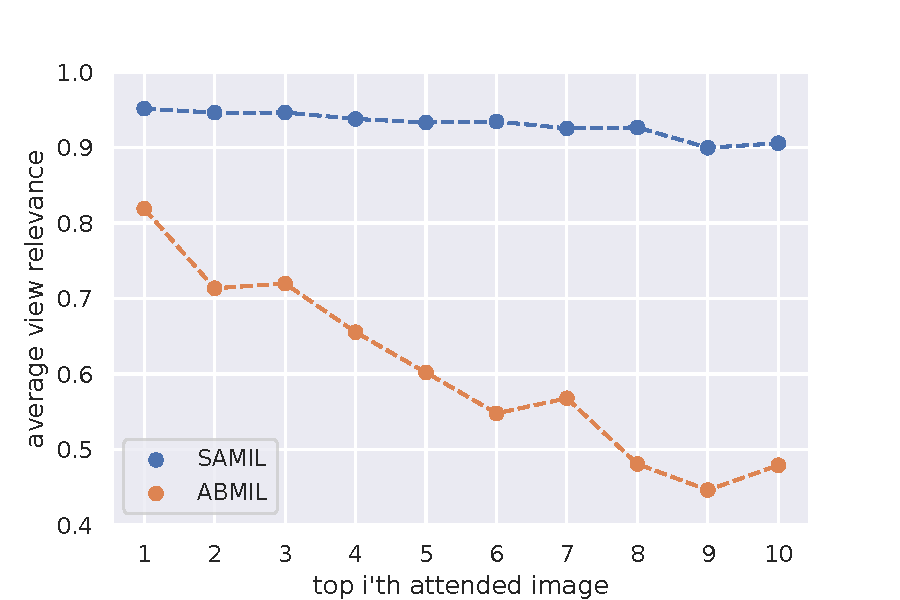
\includegraphics[width=0.32\textwidth]{figures/Attention_View_Alignment/data_seed0.pdf}
    &
    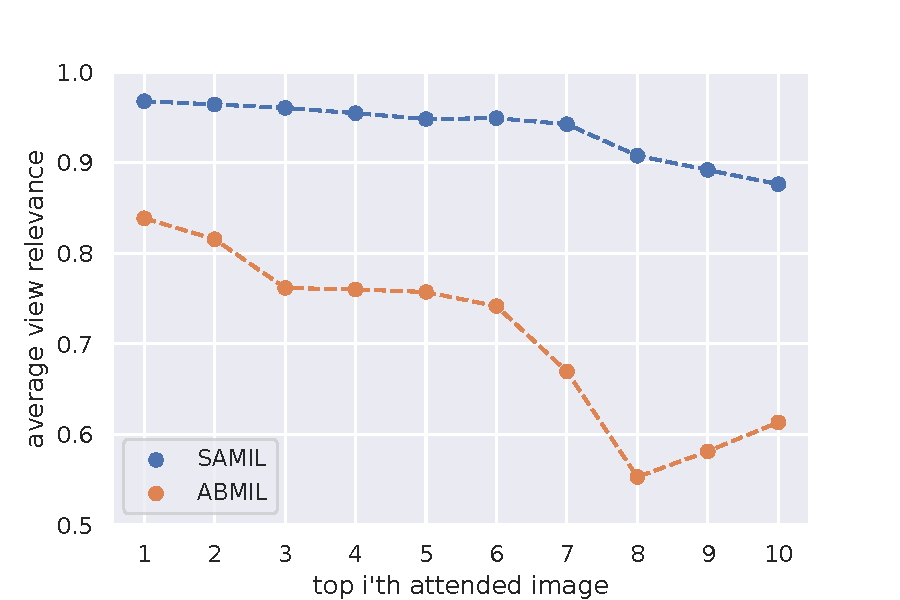
\includegraphics[width=0.32\textwidth]{figures/Attention_View_Alignment/data_seed1.pdf}
    &
    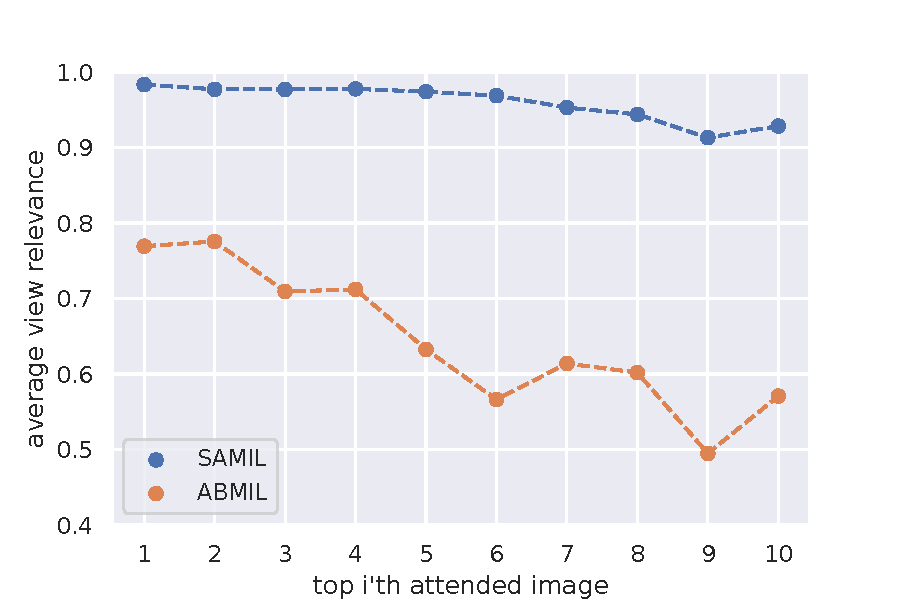
\includegraphics[width=0.32\textwidth]{figures/Attention_View_Alignment/data_seed2.pdf}
    \end{tabular}	
    \caption{
    Predicted view relevance of top-ranked images by attention (higher is better).
    %Showing the attention weights and view relevance alignment across all studies in the test set for multiple train/test splits. 
    Supervised attention (SAMIL, ours) outperforms off-the-shelf ABMIL by wide margin across all 3 splits.
    The x-axis indicates a rank position of images within an echo study when sorted by attention (1 = largest $a_k$, 2 = second largest, etc.). The y-axis indicates the average view relevance (across studies in test set) assigned by view classifier $v(x)$ to image $x$ at rank $k$. 
     }
    \label{fig:Attention_View_Alignment}
\end{figure}

% Concretely, clinicians use clinically relevant views (PLAX and PSAX) to make AS grading. Similar our model  to make the predictions based on relevant views from each TTE studies. \todo{elaborate/cite paper how this help gain trust from clinicians}.


\subsection{Ablation evaluations of attention and pretraining}

\begin{table}[!h]
\parbox{.45\linewidth}{
\centering
    \begin{tabular}{l|rrr|c}
	    & \multicolumn{4}{c}{Test Set Bal. Accuracy} \\
     Method & 1 & 2 & 3 & average \\
    \hline
    ABMIL             & 58.5 & 60.4 & 61.6 & 60.2 \\
    ABMIL Gate Attn.  & 57.8 & 62.6 & 59.8 & 60.1  \\
    SAMIL no pretrain & 72.7 & 71.6 & 73.5 &\textbf{72.6}
    \end{tabular}
    \caption{Ablation of \textbf{attention} strategies on TMED2. Showing balanced accuracy for AS severity (higher is better) on the test set across splits. All use ~2.3 M parameters.
    }%endcaption
    \label{tab:View Regularization ablation}
}%endparbox
\hfill 
\parbox{.45\linewidth}{
    \centering
    \begin{tabular}{l|rrr|c}
	          & \multicolumn{4}{c}{Test set Bal. Accuracy} \\
     Method & 1 & 2 & 3 & average \\
    \hline
    
    SAMIL no pretrain & 72.7 & 71.6 & 73.5 & 72.6 \\
    SAMIL w/ img-CL & 71.2 & 67.0 & 75.8 & 71.4 \\
    SAMIL           & 75.4 & 73.8 & 79.4 & \textbf{76.2}
    \end{tabular}
    \caption{Ablation of \textbf{pretraining} strategies on TMED2. Reporting balanced accuracy for AS severity (higher is better) on the test set across splits. All use ~2.3 M parameters.
    %Our proposed SAMIL uses study-level contrastive learning (CL), which we compare to commonly-used image-level CL and no pretraining at all.
    }%endcaption
    \label{tab:Pretraining strategy ablation}
}%endparbox
\end{table}


The effectiveness of the supervised attention is evident in Table~\ref{tab:View Regularization ablation}. SAMIL achieves an improvement of over 12\% compared to ABMIL, the model it builds upon, even without self-supervised pretraining.

To understand what SAMIL's built-in study-level (aka bag-level) pretraining adds, we compare to the regular approach of image-level self-supervised pretraining and without pretraining at all. Tab.~\ref{tab:Pretraining strategy ablation} shows that naively using image-level pretraining does not improve AS diagnosis performance, while our proposed study-level pretraining strategy successfully delivers gains.


% \begin{table}[!h]
%     \centering
%     \begin{tabular}{l|l|rrr|c|c}
% 	    & & \multicolumn{3}{c}{Split-specific Test Set} & & \\
%      Method & parameters & 1 & 2 & 3 & average \\
%     \hline
%     ABMIL             & 2.25 M & 58.51 & 60.39 & 61.61 & 60.17 \\
%     ABMIL Gate Attn.  & 2.31 M & 57.83 & 62.60 & 59.79 & 60.07  \\
%     SAMIL no pretrain & 2.31 M & 72.72 & 71.60 & 73.46 &\textbf{72.59} \\
%      \\
    
%     \end{tabular}
%     \caption{Ablation of attention strategies on TMED2 AS diagnosis. Showing balanced accuracy on the test set across multiple train/test splits.
%     }%endcaption
%     \label{tab:View Regularization ablation}
% \end{table}

% \begin{table}[!h]
%     \centering
%     \begin{tabular}{l|l|rrr|c|c}
% 	    & & \multicolumn{3}{c}{Split-specific Test Set} & & \\
%      Method & parameters & 1 & 2 & 3 & average \\
%     \hline
    
%     SAMIL no pretrain & 2.31 M & 72.72 & 71.60 & 73.46 & 72.59 \\
%     SAMIL w/ Image CL & 2.31 M & 71.24 & 67.04 & 75.84 & 71.37 \\
%     SAMIL            & 2.31 M & 75.41 & 73.78 & 79.42 & \textbf{76.20} \\
    
%     \end{tabular}
%     \caption{Ablation of SSL pretraining strategies on TMED2 AS diagnosis.  Showing balanced accuracy on the test set across multiple train/test splits.
%     Our proposed SAMIL uses study-level contrastive learning (CL), which we compare to commonly-used image-level CL and no pretraining at all.
%     }%endcaption
%     \label{tab:Pretraining strategy ablation}
% \end{table}











